\documentclass[12pt,titlepage,french]{article}
\usepackage{babel}
\usepackage{graphicx}
\usepackage[margin=2.5cm]{geometry}

\usepackage[hidelinks]{hyperref}
\usepackage{tabularx}
\usepackage[utf8]{inputenc}
\usepackage[T1]{fontenc}
\pagestyle{plain}

\usepackage{booktabs,makecell,tabu}
\usepackage{comment}
\renewcommand\theadfont{\bfseries}

\linespread{1.5}

\newcounter{firstbib}

\begin{document}
%\renewcommand{\thesection}{\arabic{section}} % utilisé pour spécifier la numérotation des sections

\begin{titlepage}
\newcommand{\HRule}{\rule{\linewidth}{0.5mm}}
\center

  
\includegraphics[width=0.45\textwidth]{../../ressources/img_logos/logo_polytech.png}\\[1cm]

  
\includegraphics[width=0.45\textwidth]{../../ressources/img_logos/logo_taglabs.png}


\HRule \\[0.4cm]
{ \huge \bfseries Rapport itération 4\\[0.15cm] }
Classification colorimétrique de nuages de points 3D\\
Version 1.0\\
Le \today \\
\HRule \\[1.5cm]
Ronan Collier,
Mathieu Letrone,
Tri-Thien Truong
\\[1cm]
\end{titlepage}

\tableofcontents % table des matières
\newpage
\listoffigures  % table des figures
\newpage

\section{Rappel des objectifs de l'itération}
Suite à l'itération où nous avions amélioré notre solution, nous avons voulu élargir nos types de filtrages, en utilisant d'autres espaces colorimétriques. De plus, nous avions encore des tâches en cours, que nous devions avancer/finaliser.

Les tâches que nous nous sommes fixées sont les suivantes :

\begin{itemize}
  \item Intégration de fausses couleurs
  \item Revoir la marge d'erreur du filtrage RGB
  \item Terminer la nouvelle méthode de segmentation
  \item Toon mapping \newline
\end{itemize}

\section{Production / réalisation durant l'itération}

Nous développerons ici chaque objectif que nous nous sommes fixé pour cette itération.

\subsection{Intégration de fausses couleurs}

Lors de l'élaboration du cahier des charges avec le client, une des tâches qui nous a été confié était l'élaboration de fausses couleurs dans un nuage de points en intensité de gris. \newline

Après la première itération, nous avons fait le choix de réaliser notre projet avec un plugin sur le logiciel CloudCompare. Nous n'avions pas pris en compte le fait que le logiciel avait déjà un système de fausses couleurs intégré. \newline

Cette tâche n'est donc plus d'actualité par rapport à ces choix d'implémentation. Nous avons donc décidé de remplacer cette tâche par une nouvelle, qui consiste à l'élaboration d'un nouvua type de filtrage, en utilisant l'espace colorimétrique HSV (Hue - Saturation - Value).

\subsection{Filtrage HSV}

Nous avons pu faire face aux limites du filtrage RGB, où il est difficile d'établir des bornes de couleurs en utilisant uniquement les trois composantes de Rouge, Vert et Bleu. \newline

L'espace colorimétrique HSV nous offre un autre moyen de définir les couleurs .  La teinte (Hue) va nous permettre de définir la couleur du point, entre 0 et 360 degrés. La saturation et la valeur, en pourcentage, nous donne respectivement des informations sur la pureté de la couleur (0 est égal à pas de couleur, donc en nuance de gris entre le blanc et le noir, et 100 pour une couleur vive), et l'intensité lumineuse (0 pour du noir, 100 pour une couleur très claire). \newline

Afin d'obtenir ces valeurs, il nous fallait convertir les valeurs RGB, en HSV. L'algorithme de conversion est disponible sur de nombreux sites internet. Un exemple de l'explication est disponible \cite{B01} ici. \newline

Une fois ceci fait, il nous était alors possible de faire notre interface pour l'utilisateur, afin d'utiliser ce nouveau type de filtrage.

\begin{figure}[!hbtp]
 \caption{\label{} Diagramme de Gantt détaillé - Sprint 4}
 \begin{center}
 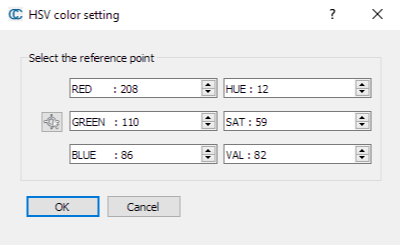
\includegraphics[width=0.75\textwidth]{./img/ui_hsv.PNG}
  \end{center}
\end{figure}

Nous pouvons donc utiliser le point picking pour sélectionner un point dont nous voulons garder dans le filtrage, puis les champs RGB et HSV se remplissent automatiquement. \newline


\subsection{Revoir la marge d'erreur du filtrage RGB}

\subsection{Terminer la nouvelle méthode de segmentation}

Un algorithme de segmentation était prévu pour être achevé à l'itération précédente. Cependant, des problèmes techniques ne nous ont pas permit d'en arriver à bout. Nous avons donc poursuivit son implémentation. Cet algorithme est séparé en deux étapes. Une première consistant à parcourir le nuage de point afin de créer des régions de couleurs similaires, et une seconde étape dite de "raffinement" afin de réunir les régions similaires. \newline
Ainsi, pour chaque point, on regarde ses voisins en ne gardant que ses voisins les plus proches (en terme colorimétrique) afin de former une région. L'algorithme complet est décrit dans une publication de l'université de \cite{B02} Whuan. 
L'algorithme est à l'heure actuelle pratiquement implémenté. Cependant, des erreurs de gestion de la mémoire sont encore présentes, ce qui empêche le plugin de démarrer correctement. La prochaine itération donnera lieu à une correction de cette erreur et à une phase de test de l'algorithme.

\subsection{Toon mapping}

Lors du sprint review de l'itération précédente, le client offrit la suggestion d'apporter une plus value dans notre solution.
L'implémentation d'un process de "Toon mapping", ce processus a pour but de restreindre le nombre de variations de couleurs au sein du nuage de points. 
Ainsi, le nuage apparaitrait de manière "cartoonesque", cela permettrait de mieux visualiser les éléments par leur couleur et pallier les variations d'intensité d'un même élément.
Ce besoin formulé dans l'itération 3, n'avait pas été prévu ni étudié en amont. Il a donc fallu réaliser des recherches sur ce domaines.

Il y a très peu de docummentation sur le toon mapping appliqué sur les nuages de points en 3D. 
Il a donc fallu faire des recherches sur des méthodes analogues dans le domaines de l'image. 
Dans l'imagerie couleur ou en nuance de gris, il existe différentes méthodes de quantification qui correspondent au principe du "toon mapping".
\newline
\begin{itemize}
    \item Octree : partition en arbre avec des branches regroupées ou abandonnées.
    \item Median-Cute : partition en "boîtes".
    \item K-moyennes local : se basant sur k-mean.
    \item Segmentation de l'histogramme.
\end{itemize}

Octree n'a pas été retenu car il demande beaucoup de mémoire et ça complexité augmente considérablement en fonction de la taille de l'image (d'autant plus que les "petits" scan compte plus d'un millions de points). Celui des k-moyenne nécessite énormément d'itérations et sa complexité fait partie des NP problème.

Ainsi, pour une première implémentation, nous avons décidé de réaliser un algorithme "simple" celui de segmentation de l'histogramme. Le fonctionnement de cet algorithme est le suivant :
\begin{itemize}
    \item On scinde l'histogramme en autant de groupe qu'on souhaite par composante
    
    (dans le cas du RGB, si on veut 3 sous-groupes par composante, on obtient 27 sous-espaces au sein de l'espace)
    \item On affecte chaque point du nuage à son cluster
    \item Pour chaque cluster, on calcule sa couleur moyenne
    \item Et on affecte cette couleur à tous les points du cluster
\end{itemize}

Actuellement, l'implémentation est terminé mais la solution est en phase de débuggage pour quelle soit totalement opérationnelle.
\section{Risques éliminés durant l'itération}


\section{Feedback}



\section{Commentaires sur l'itération}

Cette section va présenter nos ressentis sur notre itération. Cela peut correspondre à la façon dont nous avons pu gérer la charge de travail que nous avions prévu en début d'itération, des potentiels imprévus, points positifs/négatifs, et autres.

\subsection{Commentaires sur l'itération de façon générale}

L'itération a grandement été marquée par la rédaction du rapport de description, précisant le travail effectué sur le projet. Son objectif est de détailler le plus clairement possible la solution technique que nous avons apporté, afin que celle-ci puisse être améliorée et maintenue dans le cadre d'un futur projet transversal.
La rédaction de ce rapport a pris beaucoup de temps, laissant moins de créneaux horaire au développement des fonctionnalités prévues dans l'itération.
Notre objectif était de mettre en place les améliorations désirées par le client, ce que nous avons fait.

\subsection{Commentaires sur les méthodes de travail/changements de méthode}

Nous nous sommes moins fixés sur les objectifs que nous avions prévus initialement, mais plutôt sur les demandes client lors des différentes réunions.
\section{Objectifs de la prochaine itération}



%\begin{figure}[!hbtp]
% \caption{\label{} Diagramme de Gantt détaillé - Sprint 4}
% 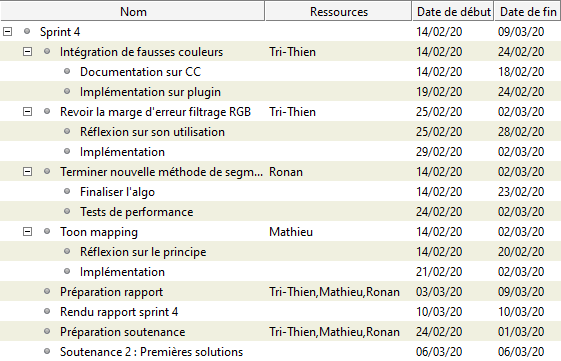
\includegraphics[width=1\textwidth]{./img/sprint_iteration_4_tableau.PNG}
% \raisebox{-1\height}
% {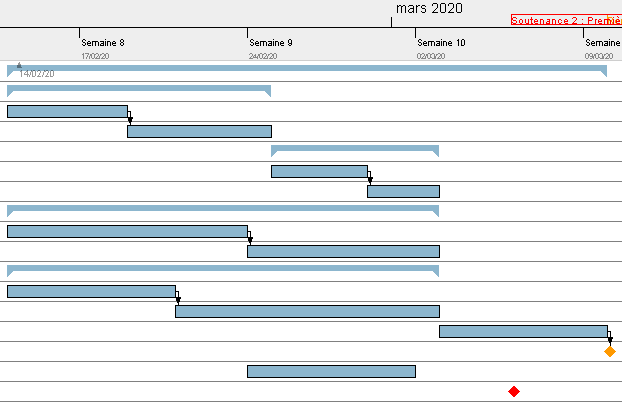
\includegraphics[width=1\textwidth]{./img/sprint_iteration_4_diagramme.PNG}} 
%\end{figure}

\section{Résumé}
\subsection{Tâches principales réalisées dans l'itération}

\subsection{Tâches principales à réaliser pour la prochaine itération}

\begin{thebibliography}{3}

\bibitem{B01} Conversion RGB - HSV: \newline
\url{https://mattlockyer.github.io/iat455/documents/rgb-hsv.pdf}

\bibitem{B02} Qingming Zhan, Yubin Liang, Yinghui Xiao, \textit{Color-based segmentation of point clouds}, 2009
\end{thebibliography}
\end{document}
